%!TEX TS-program =  xelatex
%Time-stamp: <2012-08-02 09:32:28 angenent>
\documentclass[openany,reqno]{amsbook}

\input ../preamble
\newcommand\version{1.0}
\newcommand\semester{Fall 2012}



\begin{document}

\graphicspath{{figures/}}

  %\begin{minipage}[b]{135pt}
  \hbox to135pt
  {%%%%%%%%%%%%%%%%%%%%%%%
	  \hsize135pt\parindent1pc%
	  \everydisplay{\displaywidth135pt}%
	  \sffamily\small%
	      \vbox to 108pt{%\flushleft%
	      Computing the volume of the solid you get when you revolve the
	      region $\setR$ around the $y$-axis.  A horizontal cross section
	      of the solid is a ``washer'' with inner radius $r_{\rm in}$, and
	      outer radius $r_{\rm out}$.
	
	      Another paragraph
	      \[
	      E\leq mc^2
	      \]
	    \hrule}
	    
	    \vbox to72pt{}
	    
	    \vbox to1in{\hrule%
	    
	    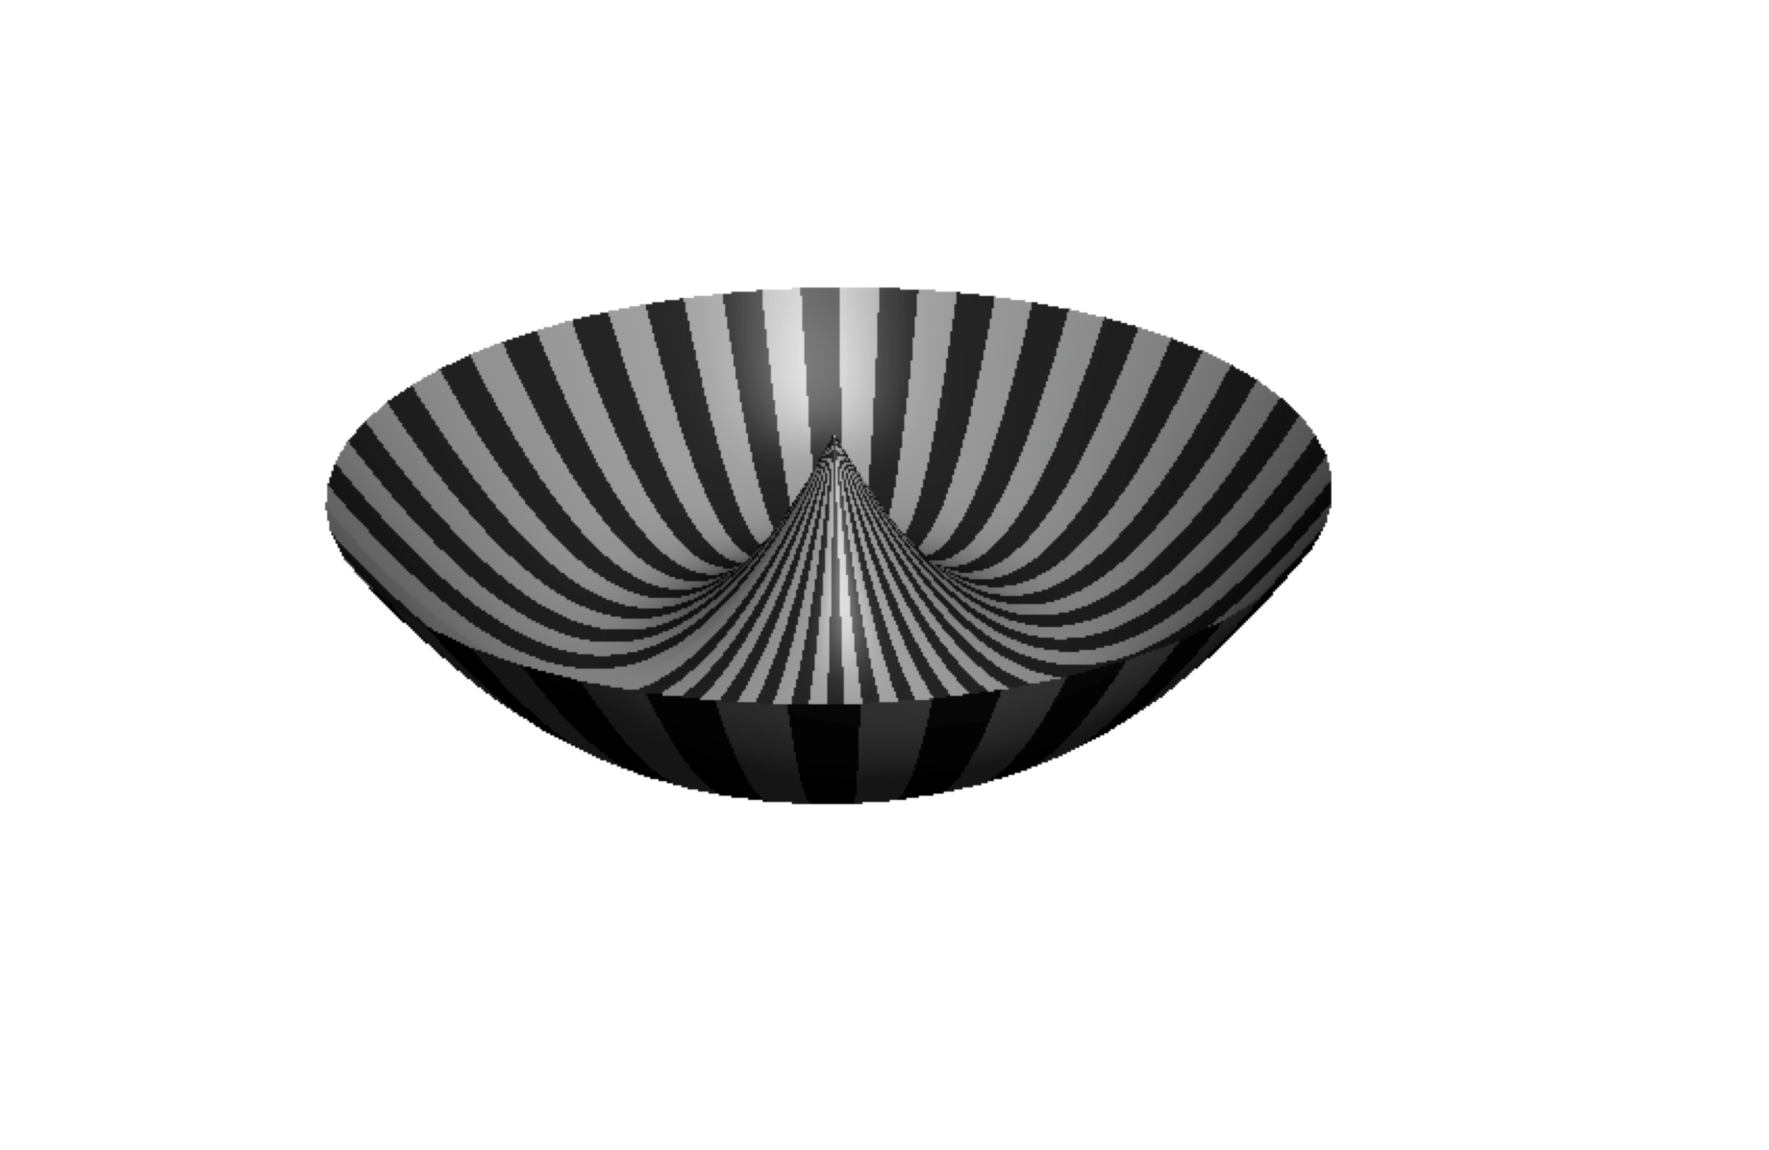
\includegraphics[width=130pt]{figures/09fancyhat.pdf} 
	    
	    \hrule}
  }%%%%%%%%%%%%%%%%%%%%%%
  %\end{minipage}\hfill
  \hbox to210pt{
    \input figures/09bowl.tex
  }
\[
E>mc^2
\]

\end{document}

%%% Local Variables: 
%%% coding: utf-8
%%% mode: latex
%%% TeX-engine: xetex
%%% End: 
